The mutation core is the final part in the genetics accelerator. The mutation core takes in a forwarded child from the crossover core as input and may perform mutation on a few selected bits before passing on the result. 

\begin{figure}[H]
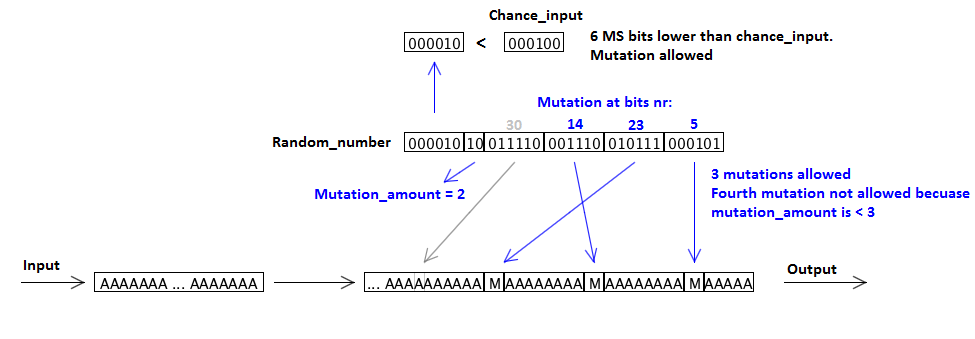
\includegraphics[width=\textwidth]{fpga/fig/mutation.png}
\caption{Mutation core fuction example}
\label{Fig_Mutation}
\end{figure}

In addition to the the 64-bit child, the mutation core also takes in a 32-bit random\_number and a 6-bit chance\_input as inputs. As it can be seen in the example in figure \ref{Fig_Mutation}, all bits that are not mutated are represented by an A, and mutated bits are represented with M. The values in each A or M can be 0 or 1, independent of each other. The value M at bit number \textit{i} is the opposite of the original value A at same bit number \textit{i} in the input.
The 6 first bits in the random\_number is compared to the chance\_input, and mutation happens only if the value of these bits are less than the chance input. For each different value in chance\_input, the user may increase or decrease the chance of mutation by about 1,5\%, or $(1 / 2^6)$. If the chance input is set to 000000, no mutation will ever happen, and the user may in this way disable the mutation core.

The next two bits in the random number (bits 25-24) are used to determine how many mutations will happen. There are 4 different values, therefore there can be 1-4 mutations.
The next 24 bits are used to determine which bits are to be mutated. 6 bits are used for finding each bit number. This is similar to what is done in the split and doublesplit functions in the crossover core. These values are numbered, representing their bit field:
\begin{itemize}
\item Nr. 1: 5-0
\item Nr. 2: 11-6
\item Nr. 3: 17-12
\item Nr. 4: 23-18
\end{itemize}
These are numbered after the amount of allowed mutation. Nr. 1 will always happen when a mutation occurs, while nr. 4 happens only when the amount\_number allows for 4 mutations.

Note that if more than one of these numbers point to the same bit to be mutated, the output M will still be the inverted from the original input. For instance, if both numbers 1 and 2 (bits 11-6 and 5-0) have the value 000110, and therefore point at bit number 6, the same mutation will still happen as if only one of these numbers were 000110. If the input bit was 1, the mutated will be 0, and vice versa.
In the example provided in figure \ref{Fig_Mutation}, the 6 first bits of the random\_number are less than the chance\_input, therefore a mutation happens. Bits 23-0 have the values 30, 14, 23 and 5. Because the value of bits 25-24 is 10 (mutation\_amount has value 2), there will be 3 mutations, and the fourth does not occur (though the figure shows where it would have occured if allowed).